%\hspace{24pt}
In this section, we verify whether our scheme balances the load more significantly than other existing methods including Strongest-Signal-First (SSF), Least-Load-First (LLF) and Cell-Breathing.

\subsection{Simulation Model}
The details of our simulation setup is shown in Table \ref{tab:Simulation-Setup}. Most parameters are configured according to existing Cell-Breathing method in literature \cite{bejerano2009cell}. We use NS3 as our simulation tool, and we set simulation time to 10000s. We totally set 20 APs, which are all support IEEE 802.11g standard. Each AP is equipped with 54 megabits per second backhaul link. These APs are located in $550 * 450 m^2$ area and they are arranged into four lines for five APs per line. The distance between two adjacent APs is set to 100 meters, and those APs are 75 meters far from the simulated area border. In order to ensure that all users are in the coverage of APs, we set the minimum transmission distance is 75 meters. To determine the transmission bit rate between users and APs, we list the relationship between SNR and bit rate in Table \ref{tab:Traffic-Bit-Rate}.

In order to build the mobility of our scenario, we use the BonnMotion tool to generate user traces. We use the Reference Position Group Mobility model (RPGM) to generate three cases of user number, which are 100, 250 and 400. Figure \ref{fig:scenario-400n} shows the scenario with 400 users in our simulated area. These users are divided into two groups and follow the group mobility. Each group brings heavy connection demand when the group moves into coverage of an AP.

%% Table 4.1
% \usepackage{booktabs}
\begin{table}[H]
\setlength{\belowcaptionskip}{15pt}
\centering
\caption{Simulation Setup}
\label{tab:Simulation-Setup}
\begin{tabular}{@{}ll@{}}
\toprule
Parameters           & Assumption                               \\ \midrule
Simulated Time       & 10000s                                   \\
Simulated Area       & 550 * 450 m\textasciicircum 2            \\
MAC Protocol         & IEEE 802.11b                             \\
Transmission Range   & {[}75, 150{]} m                          \\
Adjacent AP distance & 100 m                                    \\
AP Number            & 20                                       \\
User Number          & 100, 250,400                             \\
Mobility Model       & Reference Position Group,Mobility (RPGM) \\
Moving Speed         & {[}0.5, 1.5{]} m/s                       \\ \bottomrule
\end{tabular}
\end{table}

%% Table 4.2
% \usepackage{booktabs}
\begin{table}[H]
\setlength{\belowcaptionskip}{15pt}
\centering
\caption{Traffic Bit Rate}
\label{tab:Traffic-Bit-Rate}
\begin{tabular}{@{}ccc@{}}
\toprule
\multicolumn{1}{l}{Bit Rate (Mbps)} & \multicolumn{1}{l}{SNR(dB)} & \multicolumn{1}{l}{Distance (m)} \\ \midrule
11                                  & $\geqq 9$                     & 50                               \\
5.5                                 & $\geqq 5$                   & 80                               \\
2                                   & $\geqq 3$                    & 120                              \\
1                                   & $\geqq 1$                     & 150                              \\ \bottomrule
\end{tabular}
\end{table}
%%\clearpage

%% Figure 4.1
\begin{figure}[tbp]
\begin{center}
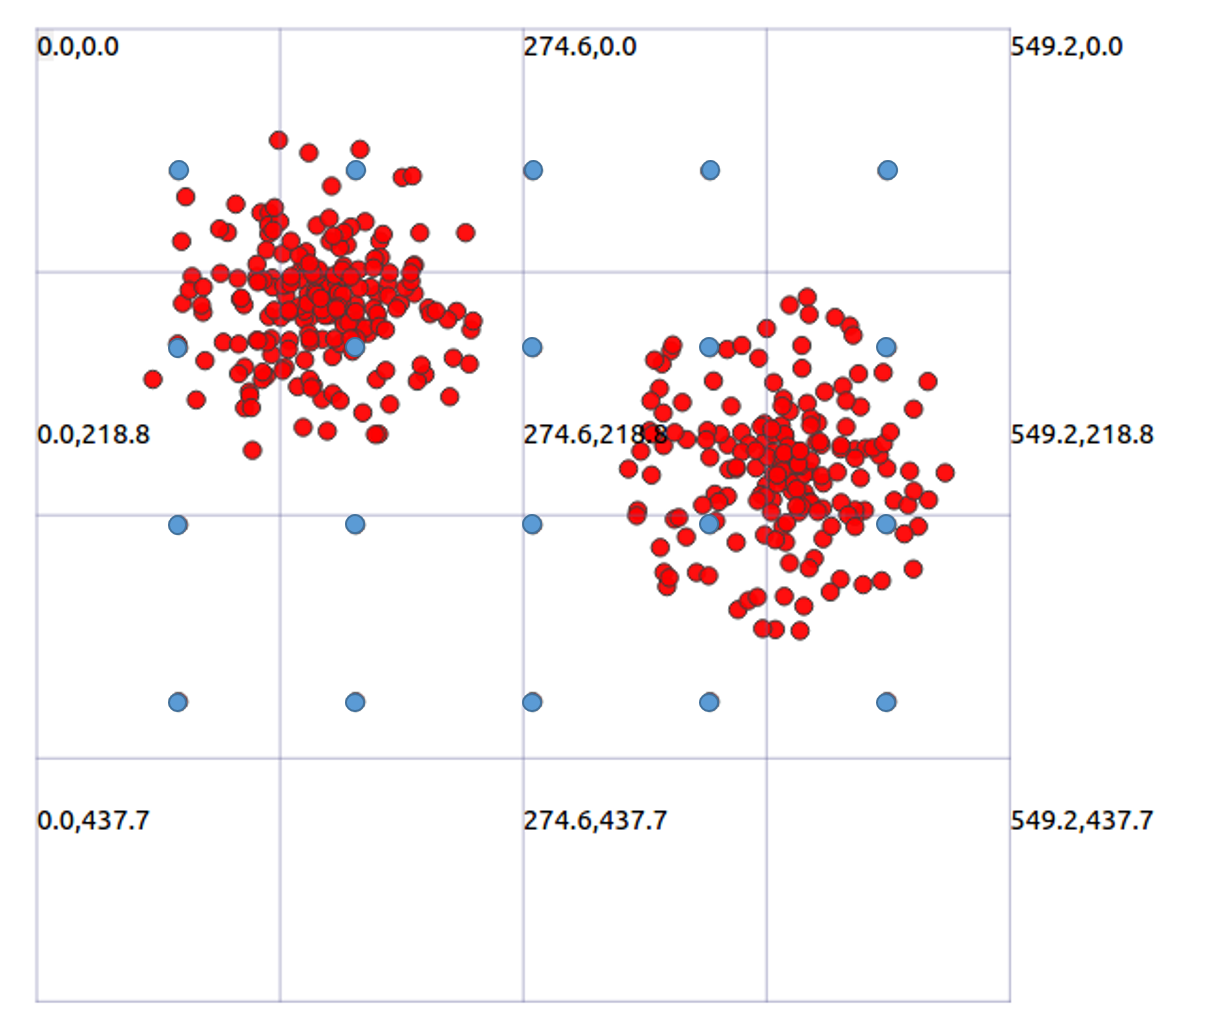
\includegraphics[width=3.4in]{images/400n.png}
\end{center}
\caption{A WLAN Scenario with 20 APs in $550*450m^2$ for NS3 Simulations (The 400 users follow the Reference Position Group Mobility model.)}
\label{fig:scenario-400n}
\end{figure}
%\clearpage

\subsection{The Performance of APs}
To measure the performance of APs, we define per second load of AP , $L_a$, to repesent the sum of associated user throughput, $L_{a,u})$. $L_{a,u}$ is the product of user bandwidth and user data rate. We assume the user bandwidth is the time interval that each AP fairly allocates the transmission time slot to its users. Users are able to transmit their data in the time slot. The user data rate can be derived from user SNR or distance with AP in Table \ref{tab:Traffic-Bit-Rate}.
\begin{align}
&L_a=\sum_{u\in{U_a}}L_{a,u}\\
&L_{a,u}=b_{a,u}*r_{a,u}\\
&b_{a,u}=\frac{1}{|U_a|}   ,|U_a|={number\ of\ users}
\end{align}

Figure \ref{fig:fig4_2a}, \ref{fig:fig4_2b} and \ref{fig:fig4_2c} show the average load of all APs with 100, 250 and 400 users respectively. The X-axis represents the index of APs, and the APs are sorted by their average load in increasing order. In the case of 100 users, we generate two groups which have average 50 users. The users are less than 50 meters from their group center. In Figure \ref{fig:fig4_2a}, we notice that the curves of our scheme, LLF and Cell-Breathing are more gently than the curve of SSF. In SSF, some APs are heavily congested and some APs are vacant.  Although the curve of Cell-Breathing is the most gently one, the sum of its average load is the least (in Table \ref{tab:Total-AP-load}). As Table \ref{tab:Total-AP-load} shows, the load of our scheme performs $11\%$ better than SSF and $347\%$ times better than Cell-Breathing. The difference between our scheme and Cell-Breathing is that we consider both the imbalance load distribution and the optimal state of all APs. Limited to the knowledge of network situation, Cell-Breathing is not able to adjust AP beacon power levels to the optimal result.

Figure \ref{fig:fig4_2b} and \ref{fig:fig4_2c} show the curves of our scheme, LLF and Cell-Breathing are more gently than the curve of SSF. In the case of 250 users, we generate five groups which have average 50 users and all users are less than 50 meters near from their group center. In the case of 400 users, we generate two groups which have average 200 users. The users of each group move around the center in 100 meters, and they bring a large amount of connection request to nearby APs. Figure \ref{fig:fig4_2c} illustrates that the gap between SSF and Cell-Breathing is smaller than the gap in Figure \ref{fig:fig4_2b}, and our scheme outperforms these two method.

%% Figure 4.2 (a)(b)(c)
\begin{figure}[tbp]
\setlength{\abovecaptionskip}{0pt}
\setlength{\belowcaptionskip}{0pt}
\begin{center}
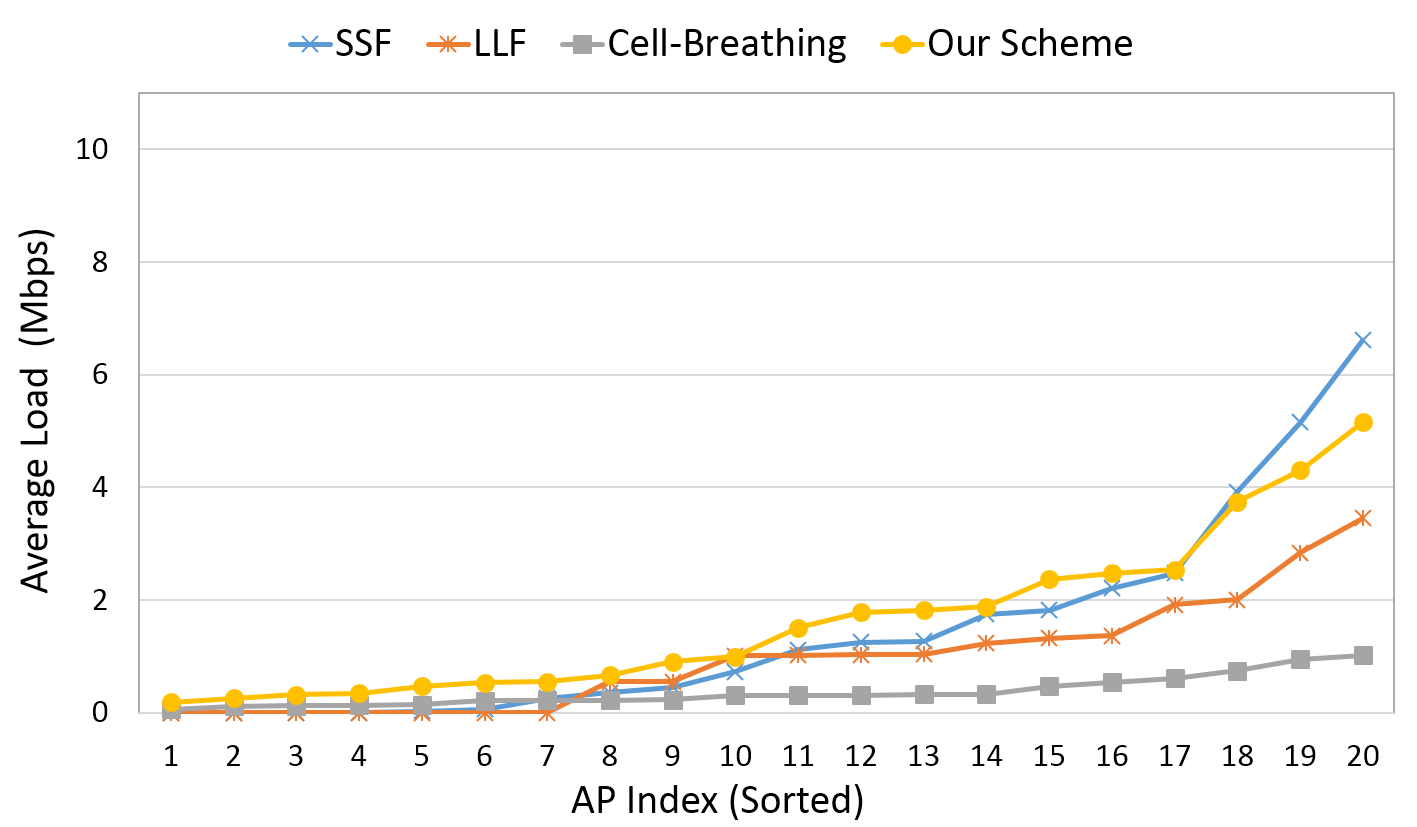
\includegraphics[width=3.4in]{images/Average_AP_load_100.png}
\end{center}
\caption{The Average Load of all APs (100 Users)}
\label{fig:fig4_2a}
\end{figure}

\begin{figure}[tbp]
\setlength{\abovecaptionskip}{0pt}
\setlength{\belowcaptionskip}{0pt}
\begin{center}
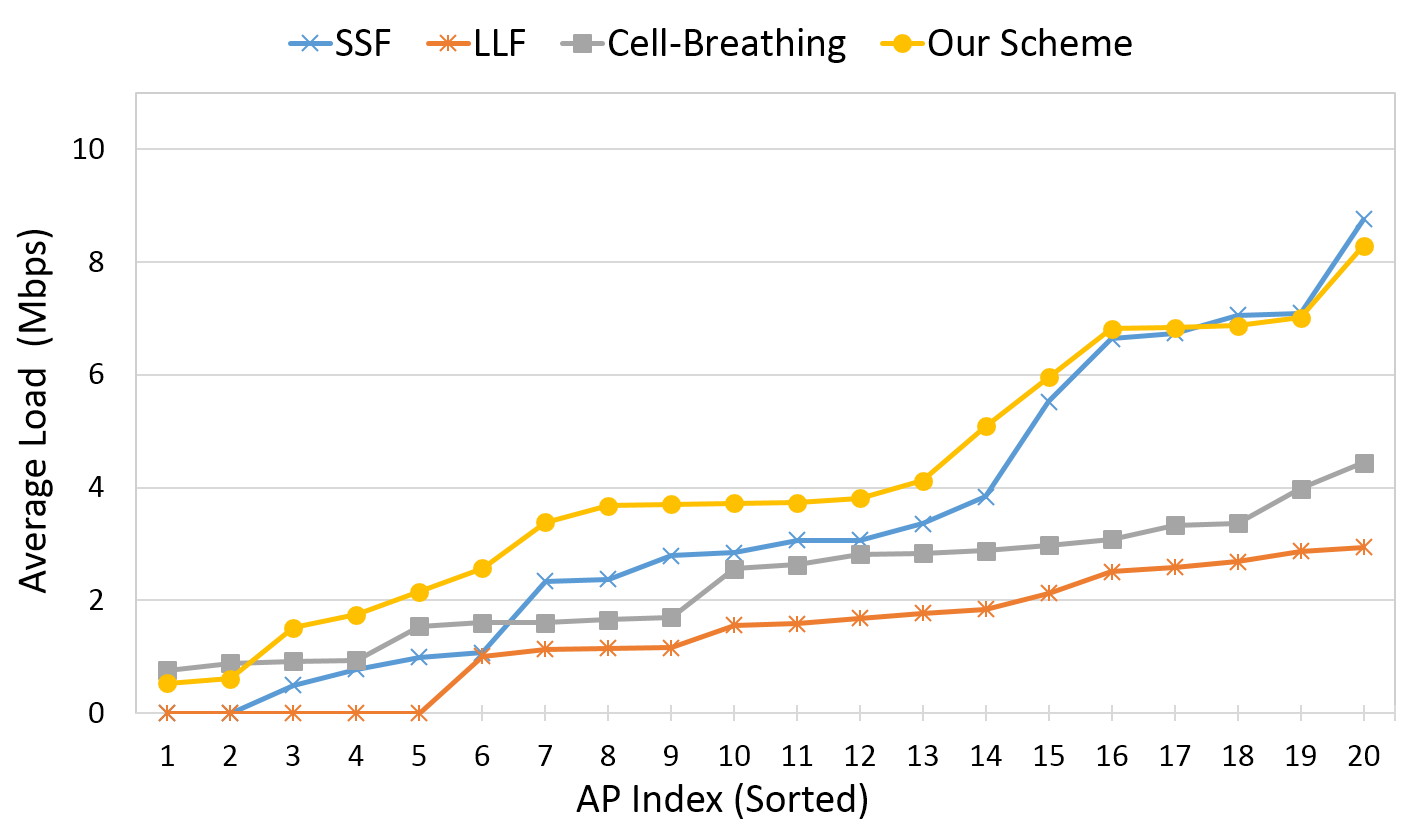
\includegraphics[width=3.4in]{images/Average_AP_load_250.png}
\end{center}
\caption{The Average Load of all APs (250 Users)}
\label{fig:fig4_2b}
\end{figure}

\begin{figure}[tbp]
\setlength{\abovecaptionskip}{0pt}
\setlength{\belowcaptionskip}{0pt}
\begin{center}
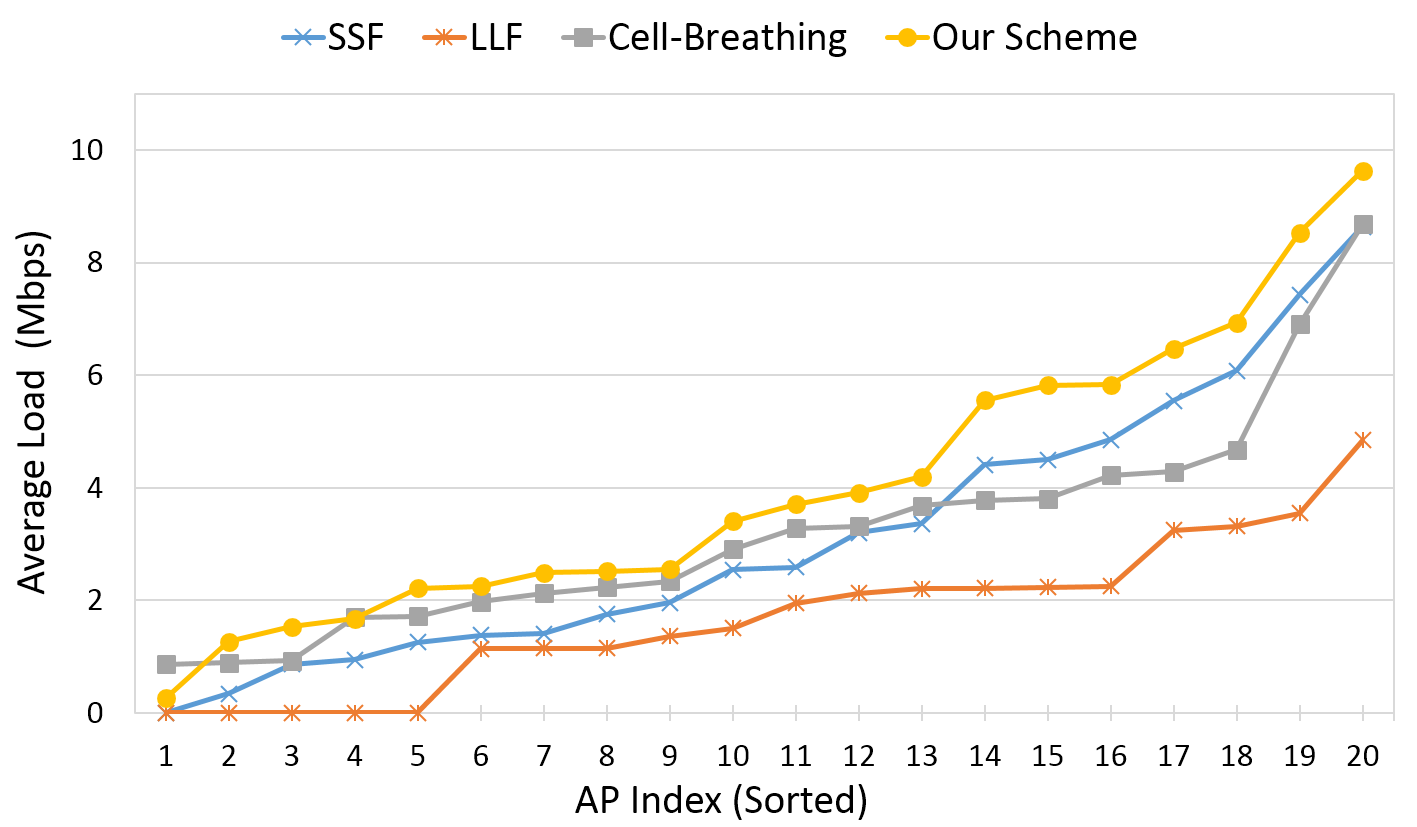
\includegraphics[width=3.4in]{images/Average_AP_load_400.png}
\end{center}
\caption{The Average Load of all APs (400 Users)}
\label{fig:fig4_2c}
\end{figure}

We calculate the average load of above three cases and compare the performance in Table \ref{tab:Total-AP-load}. As the population distribution becomes more crowded and imbalance (i.e. the number of users increases), the gap between our scheme and SSF is bigger. The load of our scheme performs $11\sim28\%$ better than SSF. Though the performance of Cell-Breathing becomes better in crowded and imbalance case, our scheme still performs $26\%$ better than Cell-Breathing. Figure \ref{fig:Total-AP-load} shows the total AP load during simulation time.

%% Table 4.3
\begin{table}[tbp]
\setlength{\belowcaptionskip}{15pt}
\centering
\caption{Summary of the AP load}
\label{tab:Total-AP-load}
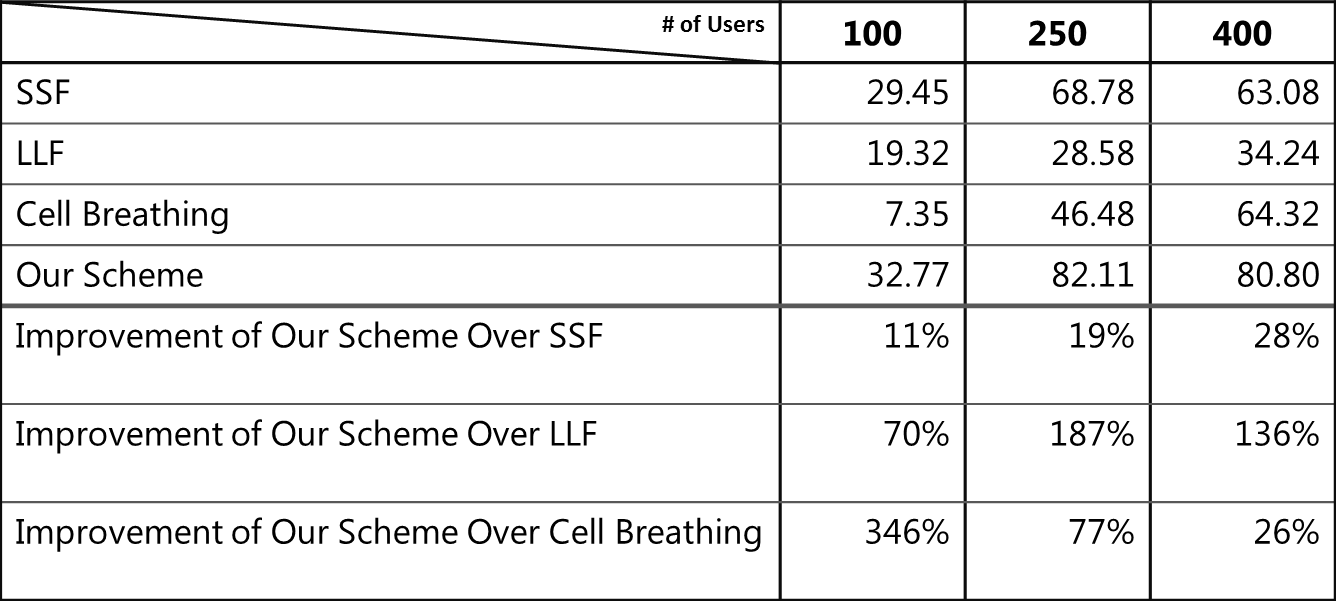
\includegraphics[width=3.4in]{images/table4_3.png}
\end{table}

%% Figure 4.3
\begin{figure}[tbp]
\begin{center}
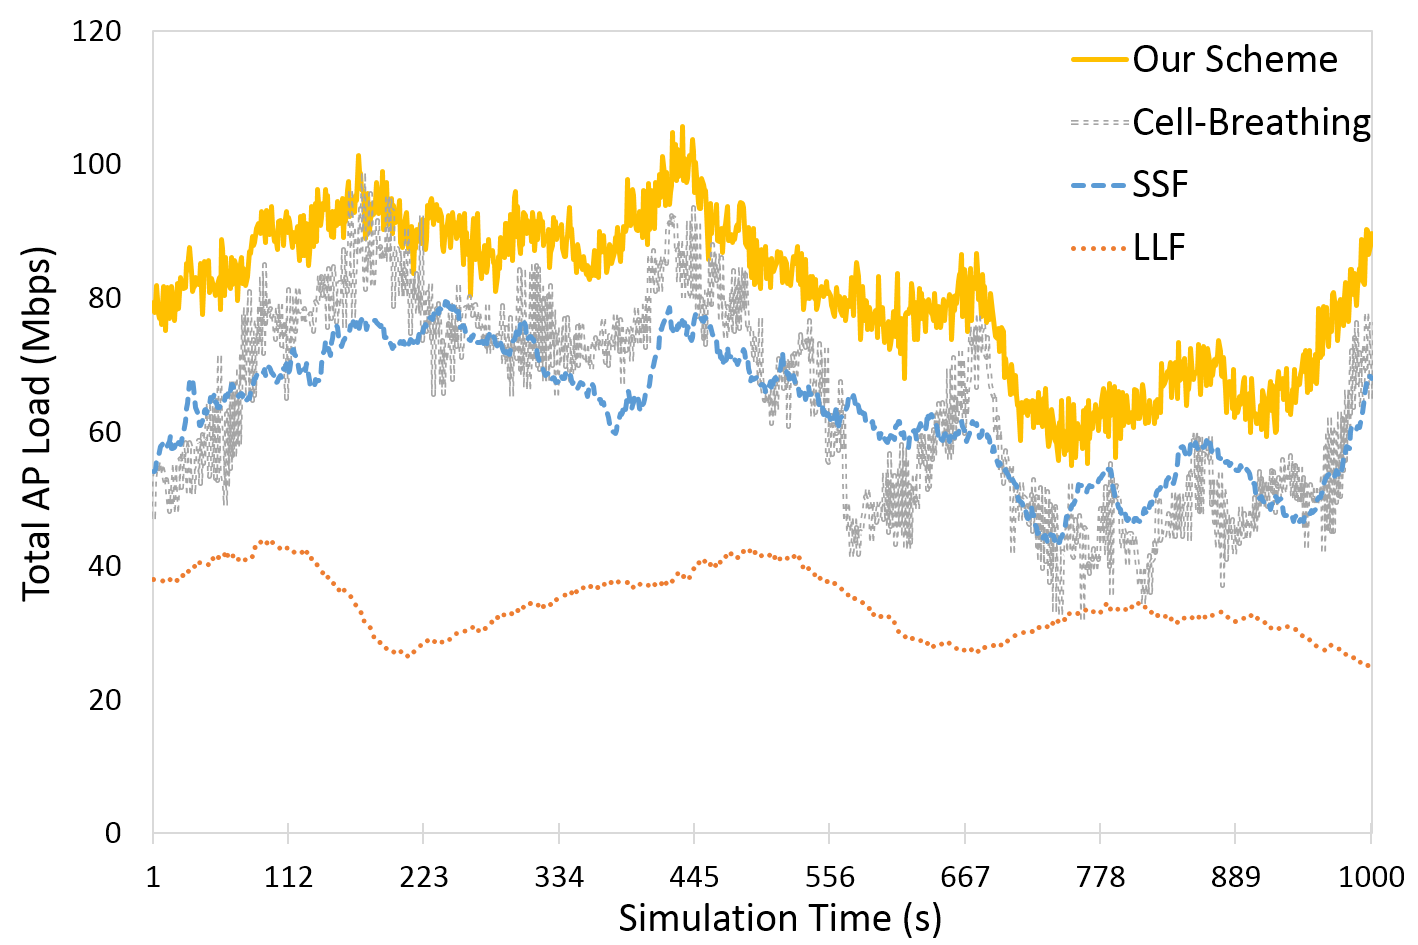
\includegraphics[width=3.4in]{images/Total_AP_load.png}
\end{center}
\caption{The Total AP Load (number of Users = 400)}
\label{fig:Total-AP-load}
\end{figure}

Figure \ref{fig:Average-user-number} illustrates the average user number of all APs in four methods. The X-axis represents the index of APs, and the APs are sorted by their average user number in increasing order. Our scheme and Cell-Breathing both balance the user number of all APs. SSF is the most imbalance method, because all users prefer to connect with the AP which has the strongest signal (i.e. the nearest AP). If there are too much users connecting to an AP at the same time, these users have poor bandwidth to transmit data.

%% Figure 4.4
\begin{figure}[tbp]
\begin{center}
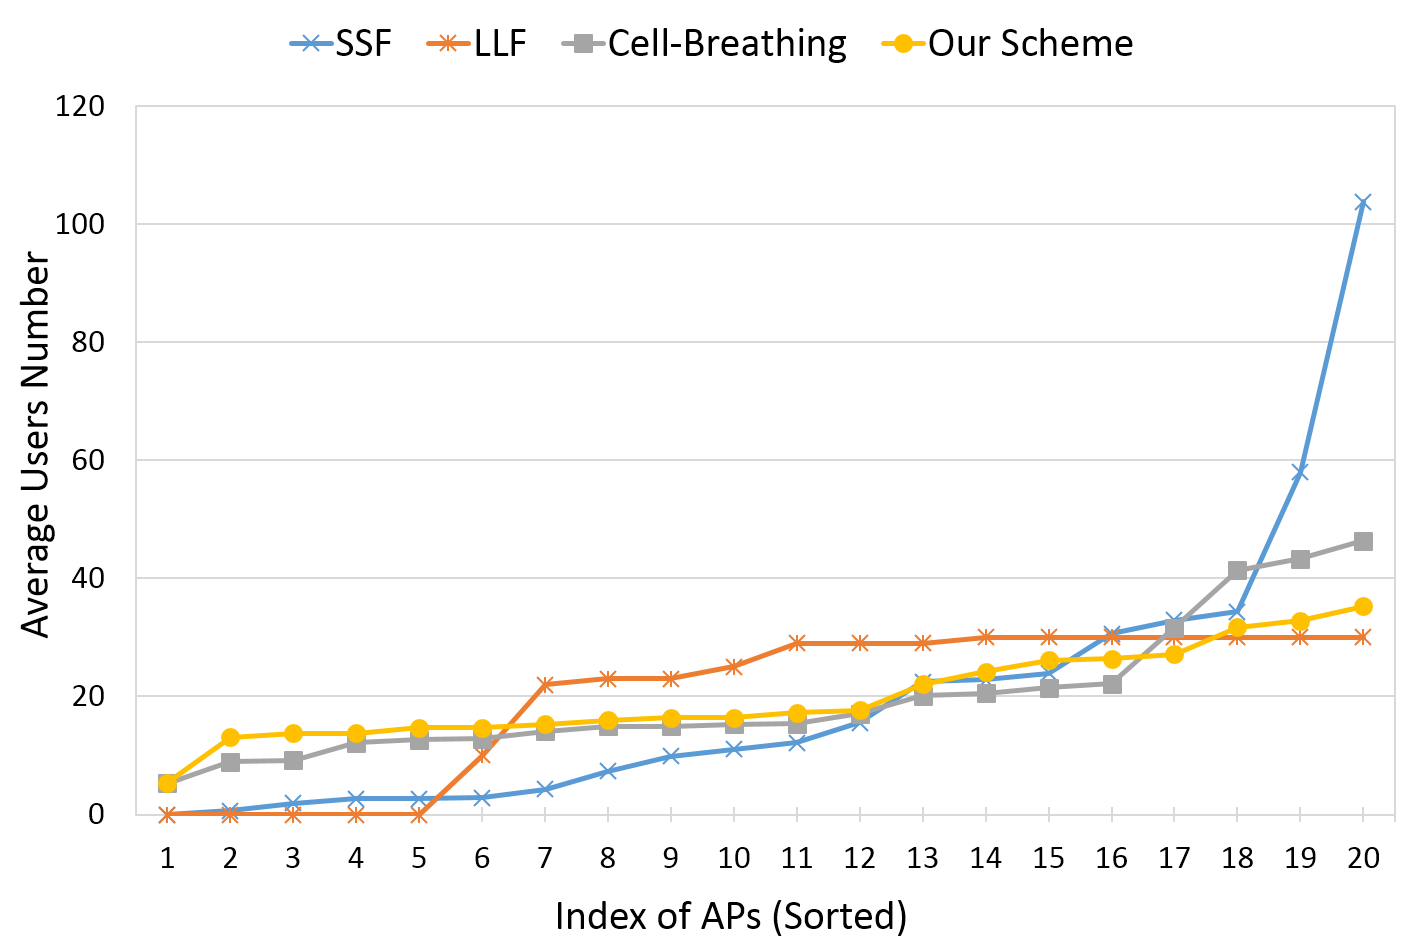
\includegraphics[width=3.4in]{images/Average_user_number.png}
\end{center}
\caption{The Average User Number of APs (number of Users = 400)}
\label{fig:Average-user-number}
\end{figure}
%\clearpage

\subsection{Impact of methods to Users}
In this subsection, we investigate the average user RSSI and average throughput with four methods. To measure the performance of user RSSI, we use the following formula and set Antenna gain 5 dBi.
\begin{equation}\label{RSSI}
  RSSI= Signal - Pathloss + Antenna_Gain
\end{equation}
In our simulation, we assume that the interference between adjacent APs can be ignored. We borrow the FSPL (Free Space Path Loss) equation of TP-Link to derive the path loss value.
\begin{equation}\label{Pathloss}
  Pathloss = 20log10(d)+ 20log10(f) + K
\end{equation}
$K$ is a constant number that depends on the unit used of distance $d$ and frequency $f$, and we set $K$ to 32.44 in our simulation.

Figure \ref{fig:Average-user-rssi} illustrates the average signal strength which user received from AP. The X-axis represents the index of users, and the users are sorted by their average RSSI in increasing order. Each average RSSI value is obtained from 10000 seconds. As a result, the users receive the highest average RSSI in SSF and the worst average RSSI in LLF. Since the users in SSF choose the highest RSSI AP to associate, and in LLF, the users intend to associate the lightest load AP. In Figure \ref{fig:Average-user-rssi}, the users in our scheme receive higher RSSI than the users in Cell-Breathing.

%% Figure 4.5
\begin{figure}[tbp]
\begin{center}
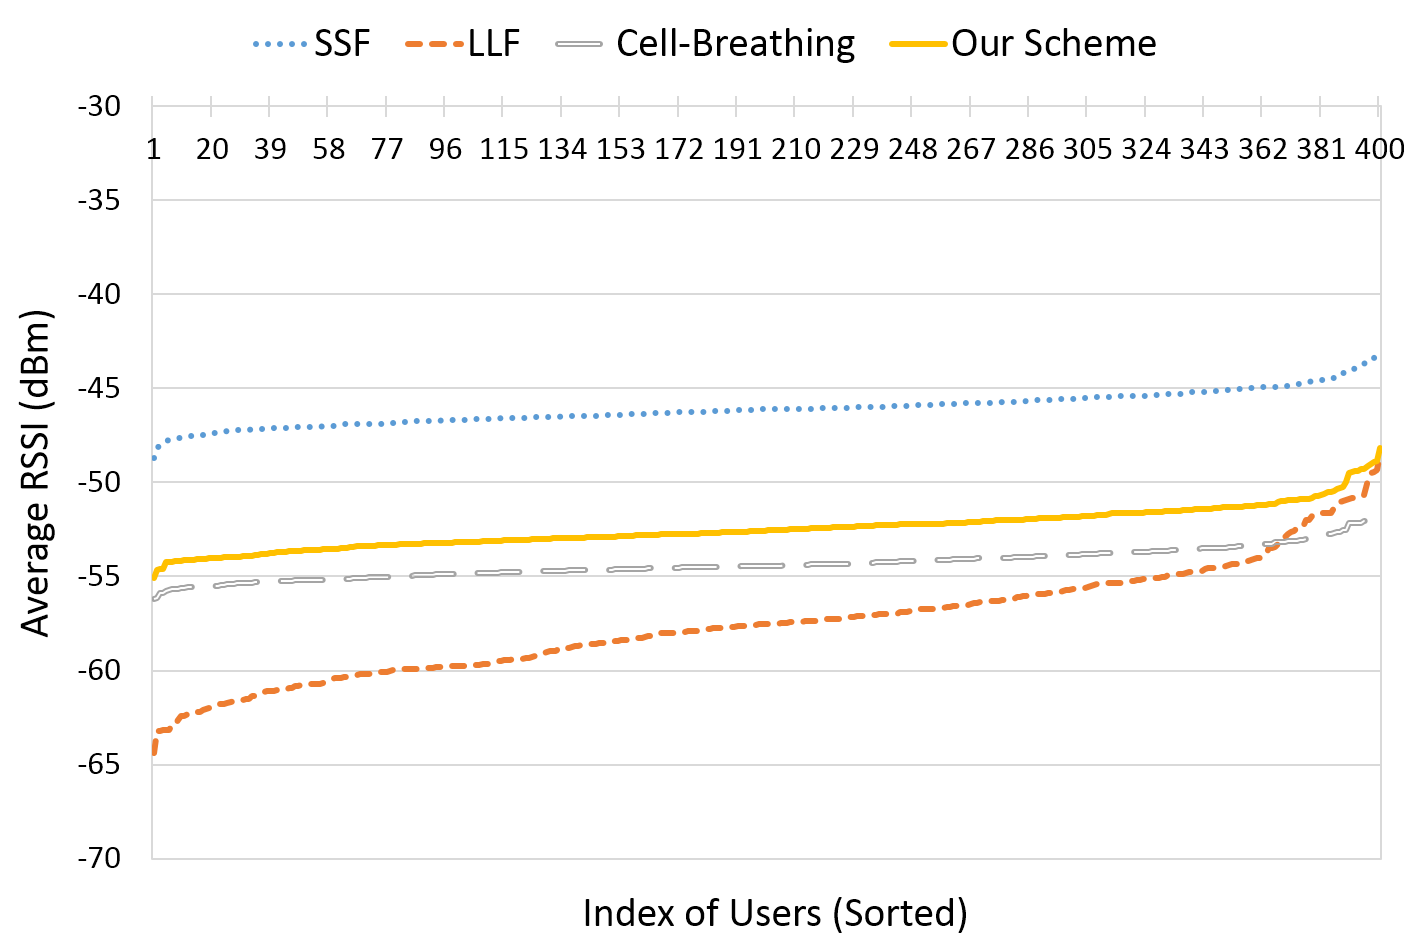
\includegraphics[width=3.4in]{images/Average_user_RSSI.png}
\end{center}
\caption{The Average RSSI of Users (number of Users = 400)}
\label{fig:Average-user-rssi}
\end{figure}

Figure \ref{fig:Average-user-throughput} shows the throughput of users. In our simulation, we assume that all users are “greedy” to use all the resource allocated from APs. However, the user usage is limited by not only user’s data rate but user’s bandwidth. In Figure \ref{fig:Average-user-throughput}, the users in our scheme have higher throughput than other methods. Due to our scheme shifts users from heavy load AP to light load AP, users can have better bandwidth and higher throughput.

We calculate the average throughput of three cases and compare the performance in Table \ref{tab:Average-user-throughput}. The load of our scheme performs $16\sim26\%$ better than SSF and performs $23\sim377\%$ better than Cell-Breathing. The performance of Cell-Breathing is very low when the population distribution is not too crowded. Overall, our scheme performs better than the other three methods in imbalanced and overcrowding environment.

%% Figure 4.6
\begin{figure}[tbp]
\begin{center}
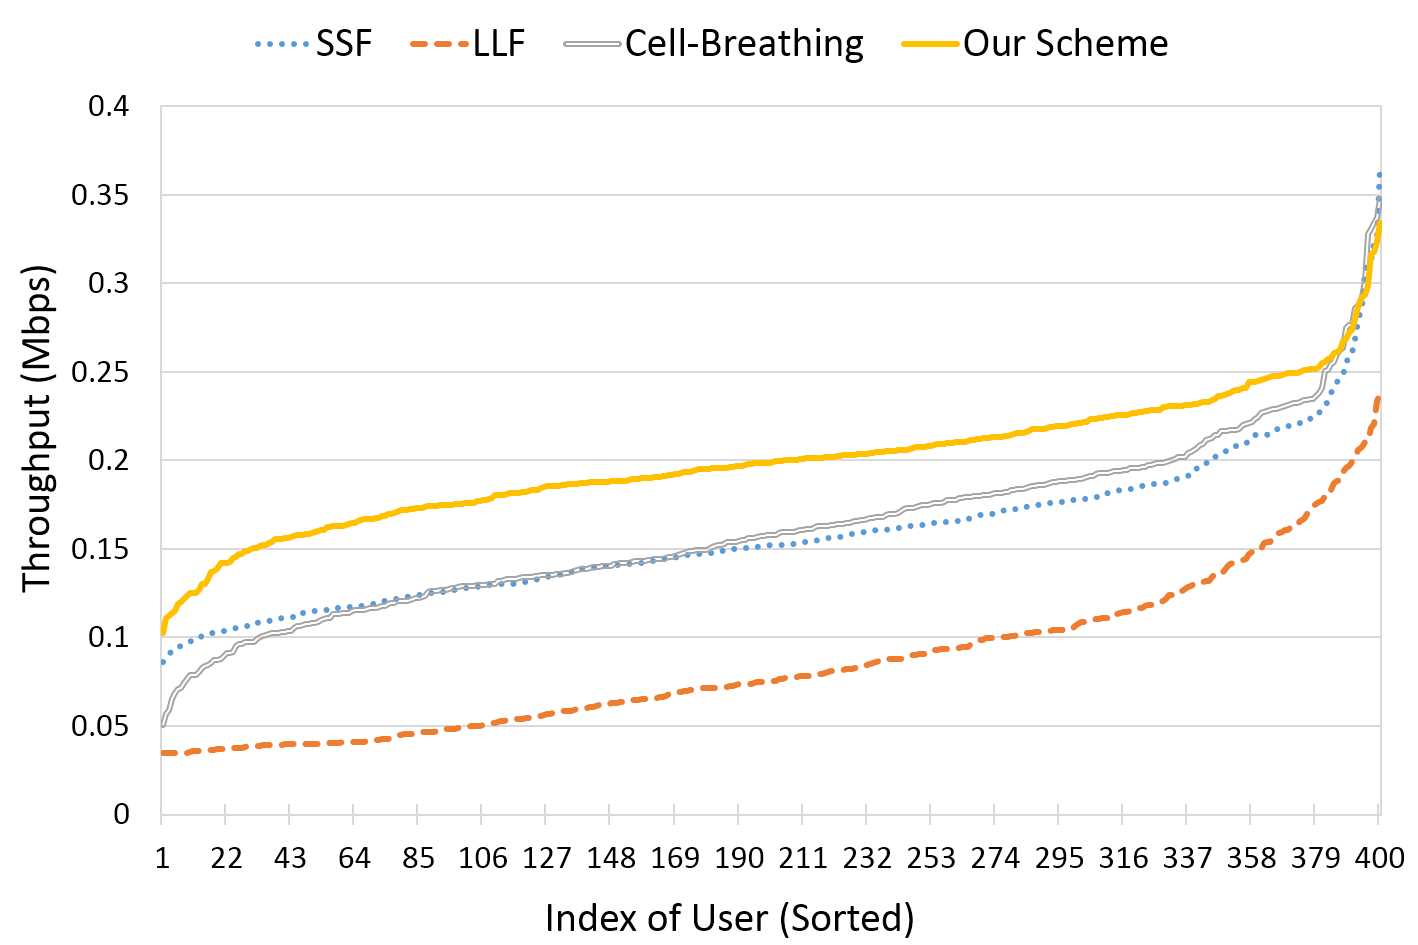
\includegraphics[width=3.4in]{images/Average_user_throughput.png}
\end{center}
\caption{The throughput of Users (number of Users = 400)}
\label{fig:Average-user-throughput}
\end{figure}

%% Table 4.4
\begin{table}[tbp]
\setlength{\belowcaptionskip}{15pt}
\centering
\caption{Summary of the User Throughput}
\label{tab:Average-user-throughput}
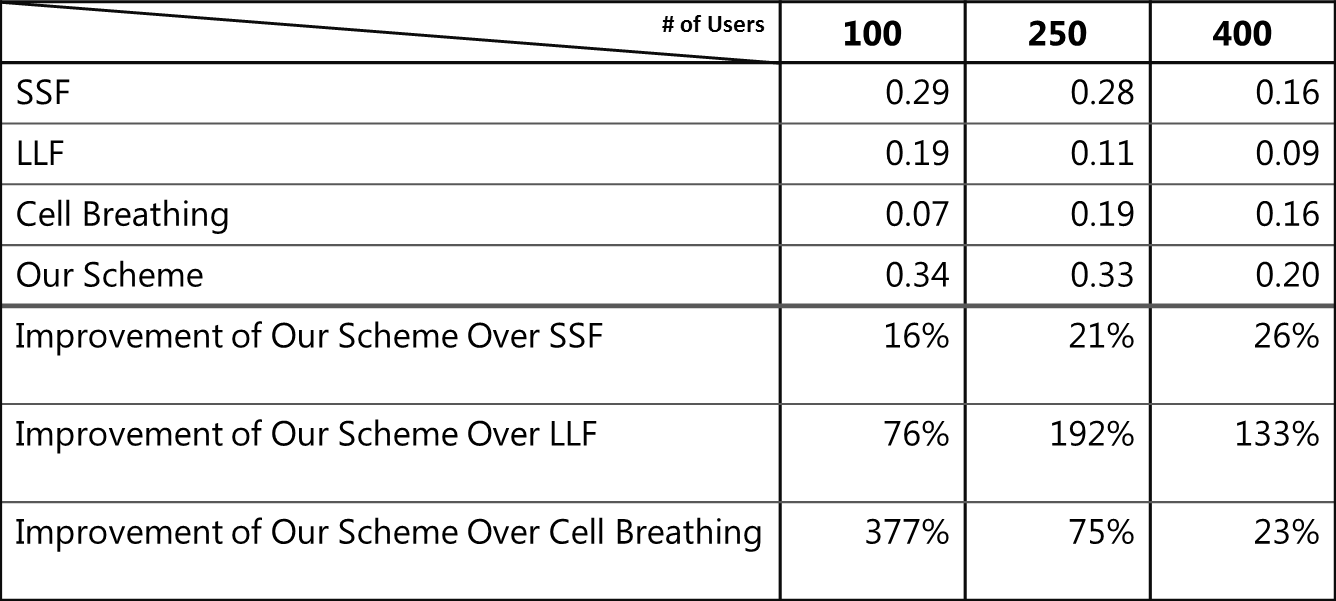
\includegraphics[width=3.4in]{images/table4_4.png}
\end{table}
%\clearpage

Figure \ref{fig:Levels} shows the impact of the power levels of our scheme. In the case of 400 users, these results show that the cases of more power levels perform better. Though the cases of more power levels take more time to compute the optimal solution, the computing time is much shorter than the people moving speed. In the figure \ref{fig:Levels}, the curve of 30 levels is almost overlapped with the curve of 50 levels, so we think that the power level ranging between 30 and 50 is suitable.

%% Figure 4.7
\begin{figure}[tbp]
\begin{center}
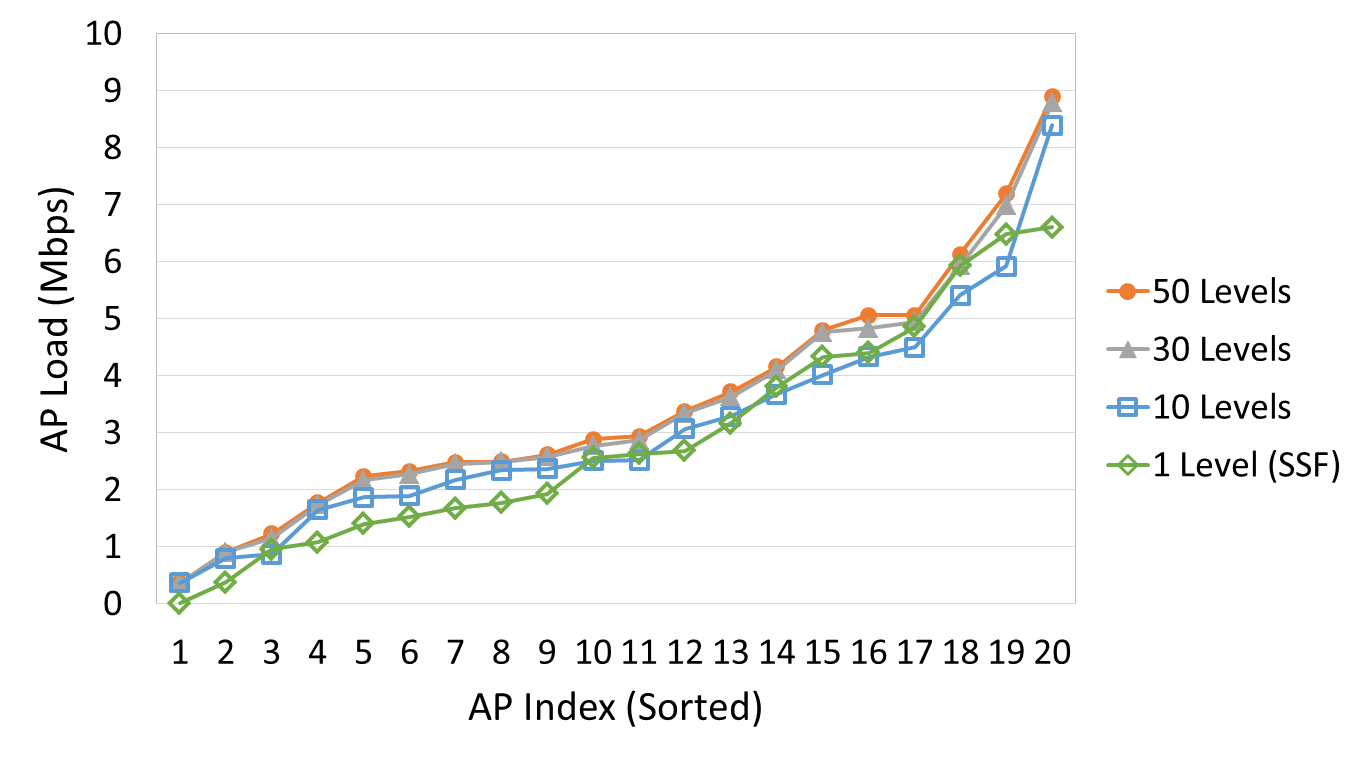
\includegraphics[width=3.4in]{images/Levels.png}
\end{center}
\caption{Impact of the Power Levels of Our Scheme}
\label{fig:Levels}
\end{figure}
% above dotto
